\documentclass[12pt,a4paper]{report}
\usepackage{graphicx}
\usepackage{amsmath}
\usepackage{fancyhdr}
\usepackage{cite}
\usepackage{framed}
\usepackage{a4wide}
\usepackage{float}
\usepackage{epsfig}
\usepackage{longtable}
\usepackage{enumerate}
\usepackage{afterpage}
\usepackage{multirow}
\usepackage{ragged2e}
\usepackage{gensymb}
\usepackage{amsfonts} 
\usepackage{tabularx}
% \documentclass[letterpaper, 11pt]{article} % For Letter size
\usepackage{booktabs}
\usepackage[utf8]{inputenc}
\usepackage[T1]{fontenc}
\usepackage[margin=2.5cm]{geometry} % Adjust the margin as needed
\usepackage{setspace} % For adjusting line spacing
\onehalfspacing % Set line spacing to one-and-a-half
\usepackage{setspace}           
\usepackage{float}
\usepackage{txfonts}
\usepackage{lipsum}

\newcommand{\Usefont}[1]{\fontfamily{#1}\selectfont}

\usepackage{lscape} % for landscape tables
\renewcommand{\baselinestretch}{1.7} 

\usepackage{blindtext}
\usepackage{xpatch}
\usepackage{url}

\usepackage{subcaption}
\usepackage{textcomp}
\usepackage{tikz}
\usetikzlibrary{arrows.meta,fit,positioning}

\linespread{1.5}
\usepackage[intoc, english]{nomencl}
\hyphenpenalty=5000
\tolerance=1000

% ******* References config *********
\bibliographystyle{IEEEtran}   % On some TeX systems this works
%\bibliographystyle{ieeetr}      % While on others this works
\renewcommand{\bibname}{References}

%*******************************************************************
%                        Header and Footer   
% Not required in technical reports. Please leave it commented.
%*******************************************************************
%\pagestyle{fancy}
%\fancyhead{}
%\renewcommand\headrulewidth{0.1pt}
%\fancyhead[L]{\footnotesize \leftmark}
%\fancyhead[R]{\footnotesize \thepage}
%\renewcommand\headrulewidth{0pt}
%\fancyfoot[R]{\small TKM College of Engineering}
%\renewcommand\footrulewidth{0.1pt}
%\fancyfoot[C]{2025 - 2026}
%\fancyfoot[L]{\small Title of the Project}

%*********************Figures*****************************
% Save all figures in the folder figures and include them in your 
% report using the command \includegraphics{figure-name}
\graphicspath{{figures/}}

% Helper: inserts the figure if the file exists in figures/, otherwise a
% labelled placeholder box, so the report compiles before all screenshots
% are captured. Usage: \safefig{file}{width}{caption}{label}
\newcommand{\safefig}[4]{%
\begin{figure}[!htbp]
\centering
\IfFileExists{figures/#1}{\includegraphics[width=#2\textwidth]{#1}}{%
\fbox{\parbox[c][4cm][c]{0.8\textwidth}{\centering Insert figure:\\ \texttt{\detokenize{#1}}}}}
\caption{#3}
\label{#4}
\end{figure}}
% figure files can be in jpeg,jpg, png or pdf formats
%*******************************************************************

\raggedbottom
\begin{document}


%****The entries in this section are to be filled in by the student with appropriate values *************
% These values are used throughout the report 

\gdef \title{Customer Churn Prediction Using Machine Learning and MLOps} % Project title
\gdef \dept{Centre for Artificial Intelligence} %Department
\gdef \degree{Master of Technology} %degree
\gdef \branch{Artificial Intelligence} %branch
\gdef \college{TKM College of Engineering}
\gdef \collegeplace{ Kollam}
\gdef \author{ARJUN.A.V} %Project batch member 1
\gdef \rollno{M25MEAI04} % Project batch member 1 ktu id
\gdef \deptabbr{Dept.of CSE} %Dept name abbreviation

\gdef \guide{Sabeena K} %project guide
\gdef \guidedes{Assistant Professor}%project guide designation

\gdef \procordinatorA{Swathy S}% coordinator 1 
\gdef \procordinatorAdes{Assistant Professor}% coordinator 1 designation

\gdef \procordinatorB{Prof. Project coordinator 2} % coordinator 2 
\gdef \procordinatorBdes{Assistant Professor}% coordinator 2 designation

\gdef \hod{Dr. Smitha P} %Head of Department
\gdef \hoddes{Professor and Head} %HOD designation

\gdef \acadyear{2025 - 26} % Academic year
\gdef \month{MARCH 2026} %Month of Report submission
\gdef \date{07-10-2025} %Date of signing the declaration

%*******************************************************************
% The front pages. The source tex files are there in the folder
% Cover page - formatted like the Spam Detection report.
% Values come from the \gdef entries in main.tex.
\begin{titlepage}
\centering

{\LARGE \textbf{\title}}\\[1.2cm]

{\large A Course Based Project Report}\\[0.6cm]

{\large \textit{Submitted to the APJ Abdul Kalam Technological University}}\\
{\large \textit{in partial fulfillment of requirements for the award of degree}}\\[1.2cm]

{\textbf{\textit{\Large \degree}}}\\
\textbf{\textit{in}}\\
{\textbf{\textit{\Large \branch}}}\\[0.8cm]
\large by\\
\textbf{\Large \author}\\[2pt]
\textbf{\large \rollno}\\[1.2cm]
\centering
\begin{figure}[h!]
\centerline{
\includegraphics[scale=0.38]{tkmlog.png}}
\end{figure}
\vspace{0.6cm}
\textbf{\dept}\\
\textbf{\college}\\
\textbf{Kerala}\\
\textbf{NOVEMBER 2026}
\end{titlepage}
 %Unless essential Do not edit this tex file

%%********************Certificate*******************
% To print name of only the project coordinator 1 in the certificate page
\include{certificate1} 

% To print names of both the project coordinators in the certificate page
%\include{certificate2} %Please uncomment this and comment the previous line
%%***************************************************

\include{declaration} %Unless essential Do not edit this tex file

\pagenumbering{roman} 

%%********************************Abstract***********************
\chapter*{\centering ABSTRACT}
\addcontentsline{toc}{chapter}{Abstract}

\noindent Customer churn, the discontinuation of a service by an existing customer, reduces recurring revenue in the telecommunications industry. This project develops an end-to-end customer churn prediction application using the IBM Telco Customer Churn dataset of 7,043 records, of which 7,032 remained after removing 11 records with missing TotalCharges values. Numerical features were median-imputed and standardised, categorical features were imputed and one-hot encoded, and class weighting with stratified splitting addressed the class imbalance (26.58\% churners). Logistic Regression, Decision Tree and Random Forest were compared using stratified five-fold cross-validation, and Random Forest was selected for its highest mean F1-score (0.6312). A classification threshold of 0.55 was chosen on validation data. On a held-out test set of 1,407 records, the model achieved an accuracy of 76.33\%, recall of 73.26\%, F1-score of 62.20\% and ROC-AUC of 83.62\%. The model is served through a FastAPI backend and a Streamlit dashboard supporting individual and batch prediction, with experiment tracking in MLflow, containerisation using Docker and cloud deployment on Render.

\vspace{0.5cm}
\noindent\textbf{Keywords:} Customer churn, Random Forest, MLOps, MLflow, FastAPI, Streamlit, Docker. % Please type in the abstract in this tex file abstract.tex
%%***************************************************
% Default Acknowledgement page
\include{acknowledgement1}  %Unless essential Do not edit this tex file
%*******************************************************************

\thispagestyle{empty}
\newpage
    
%%**********************Table of Contents***********************
\tableofcontents
\listoffigures
% \listoftables

%%********************Body of the report**********
% Arabic numbering is used in the body of the report
\cleardoublepage
\setcounter{page}{1}
\pagenumbering{arabic}

%%********************Chapter 1**********
\chapter{Introduction}

Customer churn refers to a situation in which an existing customer discontinues a service or subscription. In the telecommunications industry, retaining existing customers is important because customer loss directly affects recurring revenue. Identifying customers who are likely to leave, before they do so, allows an organisation to plan retention actions in advance.

Machine learning provides a data-driven way to estimate this risk. Using historical customer, service, contract and billing information, a classification model can learn patterns associated with churn and estimate the probability that a given customer will leave.

This project develops an end-to-end customer churn prediction application using the IBM Telco Customer Churn dataset. Three classification algorithms, namely Logistic Regression, Decision Tree and Random Forest, are compared using stratified five-fold cross-validation, and the best model is selected. A classification threshold is tuned on validation data, and the final model is evaluated once on a held-out test set.

Beyond model development, the project integrates MLOps practices. MLflow is used for experiment tracking, Joblib for saving the trained model, FastAPI as the backend prediction API, and Streamlit for an interactive dashboard. The application is containerised using Docker and deployed on the Render cloud platform. The source code is maintained on GitHub.

The objective of this project is to predict whether a telecommunications customer is likely to discontinue the service, and to deliver this prediction through a deployed, reproducible and usable application.

%%********************Chapter 2**********
\chapter{Dataset and Exploratory Data Analysis}

\section{Dataset Description}

The IBM Telco Customer Churn dataset is used for training and evaluation. The original dataset contains 7,043 customer records and 21 columns, covering customer demographics, subscribed services, contract details and billing information. The target variable is \texttt{Churn}, which takes the values \texttt{Yes} or \texttt{No}.

The \texttt{customerID} column is an identifier rather than a meaningful predictive attribute and is therefore excluded from the model inputs. This leaves 19 predictive input features.

\section{Data Cleaning}

During initial inspection, 11 missing values were found in the \texttt{TotalCharges} column. These records were removed, giving a cleaned dataset of 7,032 records. No duplicate rows were found during initial inspection.

\begin{table}[!htbp]
\centering
\caption{Summary of the dataset before and after cleaning}
\begin{tabular}{lr}
\toprule
\textbf{Item} & \textbf{Value} \\
\midrule
Original records & 7,043 \\
Original columns & 21 \\
Missing values in \texttt{TotalCharges} & 11 \\
Records after cleaning & 7,032 \\
Predictive input features & 19 \\
\bottomrule
\end{tabular}
\end{table}

\section{Dataset Structure}

The cleaned dataset is divided using stratified splitting so that the churn ratio is preserved in every partition.

\begin{table}[!htbp]
\centering
\caption{Data partitions used in the project}
\begin{tabular}{lr}
\toprule
\textbf{Partition} & \textbf{Records} \\
\midrule
Development partition & 5,625 \\
\quad Development fitting subset & 4,500 \\
\quad Validation subset & 1,125 \\
Held-out test partition & 1,407 \\
\bottomrule
\end{tabular}
\end{table}

The development fitting subset is used to train models, the validation subset is used to select the classification threshold, and the held-out test set is reserved for final evaluation only.

\section{Exploratory Data Analysis}

\safefig{churn_class_distribution.png}{0.6}{Class distribution of the churn target}{fig:class_dist}

The target is imbalanced. In the cleaned dataset of 7,032 records, 5,163 customers (73.42\%) did not churn and 1,869 (26.58\%) churned; in the original 7,043-record file the split was 73.46\% and 26.54\%, the 11 removed records all belonging to the \texttt{No} class. Because of this imbalance, accuracy alone is not a sufficient measure of performance, and precision, recall, F1-score and ROC-AUC are also reported. Class weighting and stratified splitting are used to address the imbalance.

\safefig{tenure_by_churn.png}{0.7}{Customer tenure by churn status}{fig:tenure}

Churned customers are concentrated at short tenures: the largest group of churners falls in the first few months and the count declines steadily as tenure increases, whereas non-churning customers are spread across all tenures with a pronounced peak at the longest tenures (about 70 months).

\safefig{contract_churn.png}{0.7}{Churn by contract type}{fig:contract}

The churn rate is 42.7\% for month-to-month contracts, 11.3\% for one-year contracts and 2.8\% for two-year contracts, so customers on longer contracts churn far less often.

%%********************Chapter 3**********
\chapter{Methodology}

\section{Preprocessing}

A single preprocessing pipeline is built with Scikit-learn and is saved together with the model so that exactly the same transformations are applied at prediction time.

\begin{itemize}
\item Numerical features: median imputation followed by standardisation.
\item Categorical features: most-frequent imputation followed by one-hot encoding.
\item The one-hot encoder is configured to handle unseen categories.
\end{itemize}

\section{Handling Class Imbalance}

Class weighting is used so that the minority churn class receives greater importance during training. Stratified splitting preserves the class ratio in the development, validation and test partitions.

\section{Models Evaluated}

Three classification models were evaluated:

\begin{itemize}
\item Logistic Regression
\item Decision Tree
\item Random Forest
\end{itemize}

\section{Model Selection}

Models were compared using stratified five-fold cross-validation on the development partition, and also on the single validation split.

\begin{table}[!htbp]
\centering
\caption{Model comparison (F1-score)}
\begin{tabular}{lcc}
\toprule
\textbf{Model} & \textbf{Mean CV F1} & \textbf{Validation F1} \\
\midrule
Random Forest & 0.631234 & 0.647145 \\
Logistic Regression & 0.627339 & 0.658156 \\
Decision Tree & 0.606180 & 0.642857 \\
\bottomrule
\end{tabular}
\label{tab:model_comparison}
\end{table}

Random Forest was selected because it achieved the highest mean cross-validation F1-score. Logistic Regression obtained a slightly higher F1-score on the single validation split. Cross-validation averages performance over five folds and is therefore a more stable basis for selection than a single split, but the two models are close, and Random Forest is not the best on every measure.

\safefig{model_comparison.png}{0.7}{Comparison of the evaluated models (F1-score; vertical axis starts at 0.55)}{fig:model_comp}

\section{Threshold Selection}

The classification threshold converts the predicted churn probability into a class label. A threshold of 0.55 was selected using the validation data. The test set was not used to select the threshold.

\safefig{threshold_analysis.png}{0.7}{Threshold analysis on validation data}{fig:threshold}

On the validation data, F1-score is relatively flat across a wide range of thresholds, with precision rising and recall falling as the threshold increases. A threshold of 0.55 lies in this region and retains a recall of about 0.74 while keeping precision above 0.5.

\section{Evaluation Metrics}

Model performance is reported using accuracy, precision, recall, F1-score and ROC-AUC. With $TP$, $FP$, $TN$ and $FN$ denoting true positives, false positives, true negatives and false negatives for the churn class:

\begin{equation}
\text{Precision} = \frac{TP}{TP+FP}, \qquad \text{Recall} = \frac{TP}{TP+FN}
\end{equation}

\begin{equation}
F1 = \frac{2 \times \text{Precision} \times \text{Recall}}{\text{Precision} + \text{Recall}}
\end{equation}

ROC-AUC measures the ability of the model to distinguish the two classes across all thresholds.

\section{Experiment Tracking}

MLflow is used to track experiments, model parameters and evaluation metrics, so that different runs can be compared and reproduced.

\section{Model Saving}

The trained pipeline is saved using Joblib. The following artefacts are produced for deployment:

\begin{itemize}
\item \texttt{models/best\_model.joblib}
\item \texttt{feature\_schema.json}
\item \texttt{model\_metadata.json}
\item \texttt{threshold\_config.json}
\end{itemize}

%%********************Chapter 4**********
\chapter{Results and Deployment}

\section{Test Performance}

The selected Random Forest model was evaluated on the 1,407 held-out test records at a threshold of 0.55.

\begin{table}[!htbp]
\centering
\caption{Final test results (Random Forest, threshold 0.55)}
\begin{tabular}{lr}
\toprule
\textbf{Metric} & \textbf{Test result} \\
\midrule
Accuracy & 76.33\% \\
Precision & 54.04\% \\
Recall & 73.26\% \\
F1-score & 62.20\% \\
ROC-AUC & 83.62\% \\
\bottomrule
\end{tabular}
\label{tab:test_results}
\end{table}

\safefig{roc_curve.png}{0.65}{ROC curve on the held-out test set}{fig:roc}

\section{Confusion Matrix}

\begin{table}[!htbp]
\centering
\caption{Confusion matrix on the test set (rows: actual, columns: predicted)}
\begin{tabular}{lcc}
\toprule
 & \textbf{Predicted No} & \textbf{Predicted Yes} \\
\midrule
\textbf{Actual No} & 800 & 233 \\
\textbf{Actual Yes} & 100 & 274 \\
\bottomrule
\end{tabular}
\label{tab:confusion}
\end{table}

\safefig{confusion_matrix.png}{0.65}{Confusion matrix on the held-out test set}{fig:confusion}

Of the test records, 800 non-churning customers were correctly predicted as \texttt{No}, 233 non-churning customers were incorrectly predicted as \texttt{Yes}, 100 actual churners were missed, and 274 actual churners were correctly identified.

\safefig{feature_importance.png}{0.7}{Feature importance of the Random Forest model}{fig:feat_imp}

The most influential features are the month-to-month contract, tenure and total charges, followed by the two-year contract, absence of online security, monthly charges, fibre-optic internet service and absence of technical support. Feature importance shows how much the model relied on each feature; it does not by itself establish that a feature causes churn.

\section{System Architecture}

\begin{figure}[!htbp]
\centering
\resizebox{\textwidth}{!}{%
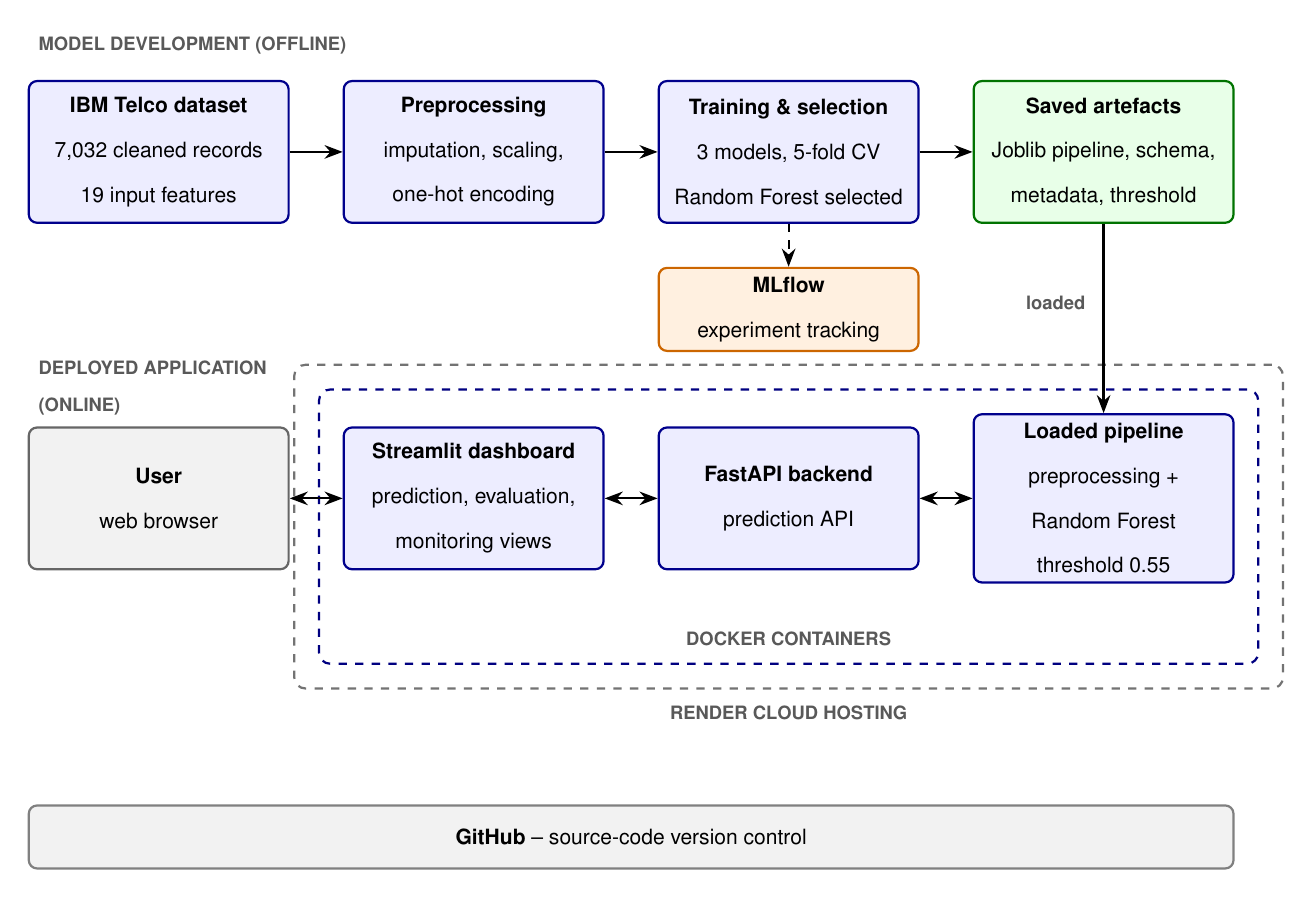
\begin{tikzpicture}[
  font=\sffamily\footnotesize,
  box/.style={rectangle, rounded corners=3pt, draw=blue!55!black, fill=blue!7, thick,
              minimum width=3.3cm, minimum height=1.8cm, align=center},
  track/.style={box, draw=orange!80!black, fill=orange!12, minimum height=0.9cm},
  store/.style={box, draw=green!45!black, fill=green!9},
  user/.style={box, draw=black!60, fill=black!5},
  arr/.style={-{Stealth[length=2.3mm]}, thick},
  darr/.style={{Stealth[length=2.3mm]}-{Stealth[length=2.3mm]}, thick},
  encl/.style={rectangle, rounded corners=4pt, dashed, thick, inner sep=0.3cm},
  lbl/.style={font=\sffamily\scriptsize\bfseries, text=black!65}
]
% ---------- model development (offline) ----------
\node[lbl, anchor=west] at (-1.65,1.35) {MODEL DEVELOPMENT (OFFLINE)};
\node[box]   (data)  at (0,0)    {\textbf{IBM Telco dataset}\\7,032 cleaned records\\19 input features};
\node[box]   (prep)  at (4,0)    {\textbf{Preprocessing}\\imputation, scaling,\\one-hot encoding};
\node[box]   (train) at (8,0)    {\textbf{Training \& selection}\\3 models, 5-fold CV\\Random Forest selected};
\node[store] (art)   at (12,0)   {\textbf{Saved artefacts}\\Joblib pipeline, schema,\\metadata, threshold};
\draw[arr] (data) -- (prep);
\draw[arr] (prep) -- (train);
\draw[arr] (train) -- (art);
\node[track] (mlf) at (8,-2.0) {\textbf{MLflow}\\experiment tracking};
\draw[arr, dashed] (train) -- (mlf);
% ---------- deployed application (online) ----------
\node[lbl, anchor=west, align=left] at (-1.65,-3.0) {DEPLOYED APPLICATION\\(ONLINE)};
\node[user] (usr)  at (0,-4.4)  {\textbf{User}\\web browser};
\node[box]  (st)   at (4,-4.4)  {\textbf{Streamlit dashboard}\\prediction, evaluation,\\monitoring views};
\node[box]  (api)  at (8,-4.4)  {\textbf{FastAPI backend}\\prediction API};
\node[box]  (pipe) at (12,-4.4) {\textbf{Loaded pipeline}\\preprocessing +\\Random Forest\\threshold 0.55};
\coordinate (dkb) at (8,-6.2);
\node[encl, draw=blue!50!black, fit=(st)(api)(pipe)(dkb)] (dock) {};
\node[lbl, anchor=south] at ([yshift=0.12cm]dock.south) {DOCKER CONTAINERS};
\node[encl, draw=black!55, fit=(dock)] (rend) {};
\node[lbl, anchor=north] at ([yshift=-0.08cm]rend.south) {RENDER CLOUD HOSTING};
\draw[darr] (usr) -- (st);
\draw[darr] (st) -- (api);
\draw[darr] (api) -- (pipe);
\draw[arr] (art) -- node[left, lbl, xshift=-1mm, yshift=2mm] {loaded} (pipe);
% ---------- source control ----------
\node[box, draw=black!50, fill=black!5, minimum width=15.3cm, minimum height=0.8cm]
      (gh) at (6,-8.7) {\textbf{GitHub} -- source-code version control};
\end{tikzpicture}}
\caption{MLOps system architecture}
\label{fig:architecture}
\end{figure}

System workflow:

\begin{enumerate}
\item The user enters customer details (or uploads a CSV file) in the Streamlit interface.
\item The inputs are sent to the FastAPI backend.
\item The saved preprocessing pipeline transforms the inputs.
\item The trained Random Forest model generates the churn probability.
\item The probability is compared with the threshold of 0.55 to obtain the predicted class.
\item The result is returned to the frontend and displayed.
\end{enumerate}

\section{System Components}

\begin{table}[!htbp]
\centering
\caption{Technologies used and their roles}
\begin{tabular}{ll}
\toprule
\textbf{Technology} & \textbf{Role} \\
\midrule
Python & Main programming language \\
Pandas / NumPy & Data handling \\
Scikit-learn & Preprocessing and model training \\
MLflow & Experiment tracking \\
Joblib & Saving the trained model \\
FastAPI & Backend prediction API \\
Streamlit & User interface and dashboard \\
Docker & Containerisation \\
Render & Cloud hosting \\
GitHub & Source-code version control \\
\bottomrule
\end{tabular}
\end{table}

\section{Application Functionality}

The Streamlit application provides the following views:

\begin{itemize}
\item Individual customer prediction
\item Batch prediction using a CSV file
\item Model evaluation and reports
\item MLflow experiment information
\item Prediction history
\item Data-drift and model-drift analysis views
\item API health information
\item Monitoring and governance views
\end{itemize}

The monitoring and governance views are monitoring-oriented analysis views. The current system does not perform fully automated production monitoring or automatic retraining.

\safefig{prediction_interface.png}{0.85}{Individual customer prediction interface (example predicted as likely to churn)}{fig:pred_ui}

The user enters the customer attributes and the interface returns the churn probability and the predicted class at the 0.55 threshold. In this example the churn probability is 58.72\%, so the customer is predicted as likely to churn.

\safefig{dashboard_overview.png}{0.85}{Dashboard overview}{fig:dashboard}

The overview page summarises the dataset size (7,032 records), the selected model (Random Forest), the test F1-score (0.622) and the ROC-AUC (0.836). The sidebar shows the model version (1.1.0) and the decision threshold (0.55).

\section{Containerisation and Cloud Deployment}

The application is containerised with Docker. The Docker configuration comprises \texttt{Dockerfile.api}, \texttt{Dockerfile.streamlit}, \texttt{Dockerfile.combined} and \texttt{compose.yaml}. The application is hosted on the Render cloud platform and can be accessed through a web browser.

\begin{itemize}
\item Deployed dashboard: \url{https://customer-churn-mlops-dashboard.onrender.com/}
\item Source code: \url{https://github.com/ajuanil9898-star/customer-churn-mlops}
\end{itemize}

\section{Challenges and Resolutions}

Challenges encountered:

\begin{itemize}
\item Class imbalance in the churn target
\item Selecting a model fairly when validation and cross-validation results differ slightly
\item Keeping preprocessing identical between training and prediction
\item Deployment environment compatibility
\end{itemize}

%%********************Chapter 5**********
\chapter{Discussion \& Conclusion}

\section{Summary}

This project demonstrates an end-to-end customer churn prediction system using machine learning and MLOps practices. Three classification algorithms were evaluated, and Random Forest was selected on the basis of cross-validation performance. On the held-out test set it achieved an ROC-AUC of 83.62\% and an F1-score of 62.20\%.

\section{Performance Analysis}

At the chosen threshold the model identifies 73.26\% of actual churners (274 of 374), which is useful when missing a churner is costly. The trade-off is a precision of 54.04\%: 233 non-churning customers were flagged as likely to churn. The threshold can be changed to trade recall against precision according to the cost of a retention action.

The difference between Random Forest and Logistic Regression is small, and Logistic Regression scored higher on the single validation split. The selection therefore rests on the more stable cross-validation result rather than on every metric.

\section{Limitations}

\begin{itemize}
\item Results are based on a single public dataset and may not transfer directly to another operator.
\item The monitoring and governance views are analysis views; automated production monitoring and automatic retraining are not implemented.
\end{itemize}

\section{Future Scope}

Future improvements include:

\begin{itemize}
\item More advanced monitoring and drift alerts
\item Automated retraining pipelines
\item Business-oriented customer retention strategies built on the predictions
\item Evaluation of additional algorithms and model-explainability methods
\end{itemize}

\section{Conclusion}

The project shows how a machine-learning model can be taken from data preparation and model comparison to a deployed application with experiment tracking, a backend API, an interactive dashboard, containerisation and cloud hosting. It provides a foundation that can be extended with stronger monitoring and retraining.

\appendix
\chapter{Web Application Screenshots}
\label{appendix:web_interface}

This appendix contains additional screenshots of the deployed web application.

\safefig{appendix_prediction.png}{0.85}{Individual customer prediction for a second example input (predicted as likely to stay).}{fig:app_pred}

\safefig{appendix_batch.png}{0.85}{Batch prediction page with CSV upload.}{fig:app_batch}

\safefig{appendix_mlflow.png}{0.85}{MLflow experiment information view in the dashboard.}{fig:app_mlflow}

\safefig{appendix_monitoring.png}{0.85}{Monitoring and governance view.}{fig:app_monitor}

\safefig{appendix_api_health.png}{0.85}{API and system health view, including Docker configuration status.}{fig:app_api}

\end{document}